\documentclass[coda.tex]{subfiles}
\begin{document}

\appendix

\section{Proof of Proposition 1}\label{appdx_proposition}

\begin{lemma}
If $V^j \in \parents^\L(V^i)$ in DAG $G^\L$ of (local) causal model $\M^\L$, and $\L \subset \mathcal{X}$, then $V^j \in \parents^\mathcal{X}(V^i)$ in DAG $G^\mathcal{X}$ corresponding to causal model $\M^\mathcal{X}$. 
\end{lemma}
\vspace{-\baselineskip}
\begin{proof}
By minimality, there exist $\{u^i, v^{-j}, v^j_1\}$ and $\{u^i, v^{-j}, v^j_2 \}$ with $v^{-j} \in \parents^\L(V^i)\setminus V^j$ for which $f^i(\{u^i, v^{-j}, v^j_1\}) \not= f^i(\{u^i, v^{-j}, v^j_2 \})$. Expand $\{v^{-j}, v^j_1\}$ and $\{v^{-j}, v^j_2\}$ to $(s_1, a_1), (s_2, a_2) \in \L$ (with any values of other components). But $\L \subset \mathcal{X}$, so $(s_1, a_1), (s_2, a_2) \in \mathcal{X}$ and it follows from minimality in $\mathcal{X}$ that $V^j \in \parents^\mathcal{X}(V^i)$.
\end{proof}

\begin{corollary}\label{corollary_sparser}
If $\L \subset \mathcal{X}$, $G^\L$ is sparser (has fewer edges) than $G^\mathcal{X}$. 
\end{corollary}\vspace{\baselineskip}

\begin{appdxProp}{1}
The causal mechanisms represented by $\G_i, \G_j \subset \G$ are independent in $\G^{\L_1 \cup \L_2}$ if and only if  $\G_i$ and $\G_j$ are independent in both $\G^{\L_1}$ and $\G^{\L_2}$, and $f^{\L_1,i} = f^{\L_2,i}, f^{\L_1,j} = f^{\L_2,j}$.
\end{appdxProp}
\vspace{-\baselineskip}
\begin{proof}

($\Rightarrow$)
If $\G_i$ and $\G_j$ are independent in $G^{\L_1 \cup \L_2}$, independence in $\G^{\L_1}$ and $\G^{\L_2}$ follows from Corollary \ref{corollary_sparser}. That $f^{\L_1,i} = f^{\L_2,i}$ (and $f^{\L_1,j} = f^{\L_2,j}$), on their shared domain, follows since each is a restriction of the same function $f^{\L_1 \cup \L_2,i}$ (or $f^{\L_1 \cup \L_2,j}$).

($\Leftarrow$)
Suppose $\G_i$ and $\G_j$ are independent in $\G^{\L_1}$ and $\G^{\L_2}$ but not $G^{\L_1 \cup \L_2}$. By the definition of independence applied to $G^{\L_1 \cup \L_2}$, we have that, without loss of generality, there is a $V_i \in \G_i, V_j \in \G_j$ with $V_j \in \parents^{\L_1 \cup \L_2}(V_i)$. Then, from the definition of minimality, it follows that there exist $(s_1, a_1), (s_2, a_2) \in \L_1 \cup \L_2$ that differ only in the value of $V_j$, and $u_i \in \textrm{range}(U_i)$ for which $f^i(s_1, a_1, u_i) \not= f^i(s_2, a_2, u_i)$. 

Clearly, if $(s_1, a_1)$ and $(s_2, a_2)$ are both in $\L_1$ (or $\L_2$), there will be an edge from $V_j$ to $V_i$ in $\G^{\L_1}$ (or $\G^{\L_2}$) and the claim follows by contradiction. Thus, the only interesting case is when, without loss of generality, $(s_1, a_1) \in \L_1$ and $(s_2, a_2) \in \L_2$. 
The key observation is that $(s_1, a_1)$ and $(s_2, a_2)$ differ only in the value of node $V_j \not\in \G_i$: since $\G_i$ is an independent causal mechanism in both $\G^{\L_1}$ and $\G^{\L_2}$ and the parents of $V_i$ take on the same values in each, we have that $f^i(s_1, a_1, u_i) = f^{i,\L_1}(s_1, a_1, u_i) = f^{i,\L_2}(s_2, a_2, u_i) = f^i(s_2, a_2, u_i)$ and the claim follows by contradiction. 
\end{proof}

\section{Additional Experiment Details}\label{sec:training_details}
This section provides training details for the experiments discussed in Section \ref{sec:experiments} as well as some additional results. Code is available at \url{https://github.com/spitis/mrl} \cite{mrl}.

\subsection{Online RL}
Here we detail the procedure used in the Online RL experiments in the Spriteworld environment.

\paragraph{Implementation} We work
with the original TD3 codebase, architecture, and hyperparameters (except batch size; see below), and focus our
efforts solely on modifying the agent’s training distribution.

\paragraph{Environment} We extend the base Spriteworld framework \cite{watters2019cobra} with (1) basic collisions (to induce a local factorization / so that a global factorization will not work), (2) a new continuous action space (2-dimensional), (3) a disentangled state renderer that returns the position and velocity of each sprite (a total of 16-dimensions in tasks with four sprites), (4) a mask renderer that returns the ground truth masking function (allows us to evaluate our masking function in Appendix \ref{sec:inferring_local_factorization}), and (5) a suite of partial and sparse reward tasks that we use for experiments. These extensions will included with the release of our code.

\paragraph{Data augmentation}
Every 1000 environment steps, we sample 2000 pairs of random transitions from the agent's replay buffer, and apply CoDA to produce a maximum of 5 unique CoDA samples per pair. We apply two forms of CoDA, using (1) an oracle / ground truth mask function that we back out of the simulator, and (2) the mask of a pre-trained transformer model (see Section \ref{sec:inferring_local_factorization}).
The mask function was trained using approximately 42,000 samples from a random policy (5/6 of 50,000, with the rest of the data used for validation). CoDA samples are added to a second CoDA replay buffer. For purposes of this experiment both buffers are have effectively infinite capacity (they are never filled). During training, the agent's batches are sampled proportionally from the real and CoDA replay buffers (this means that approximately 7/8 of the data that the agent trains on is counterfactual).

\paragraph{Baselines} 
In addition to the base TD3 agent and CoDA, we also use the transformer model that is used as a mask function to generate data by performing forward rollouts with a random policy, as in Dyna \cite{sutton1991dyna}. So that this baseline produces approximately the same number of samples as CoDA with the learned mask, we roll the model out for 5 steps from 1500 random samples from the replay buffer, again every 1000 environment steps. This produces 7500 model-based samples for every 1000 environment transitions.

Use of the transformer mask function requires setting the threshold value $\tau$, which we do by monitoring accuracy and F1 scores for sparsity prediction (as discussed in Appendix \ref{sec:inferring_local_factorization}) on validation data,
ultimately using the value $\tau = 0.05$.

\paragraph{Batch Size}
Since CoDA samples are plentiful we increase the agent's batch size from 256 to 1000 to allow it to train on more environment samples in the same number of training steps. We found that this slightly improved the performance of the base TD3 agent. An increase in batch size also allows the agent to see more of its own on-policy data in the face of many off-policy CoDA samples. 

\paragraph{Additional results in sparse reward task variants}

In addition to the partial reward tasks described in Section \ref{sec:experiments}, we also tested CoDA in four sparse reward tasks of varying difficulty. These are the same as the partial reward tasks, except that a sparse reward of 1 is granted only when \textit{all} N sprites are in their target locations. While these tasks were much harder (and perhaps impossible in the case of Place 4 due to moving sprites), as shown in Figure \ref{fig_rl_results_plot_sparse}, the CoDA agents maintain a clear advantage.


\begin{figure}[!t]
	\centering
	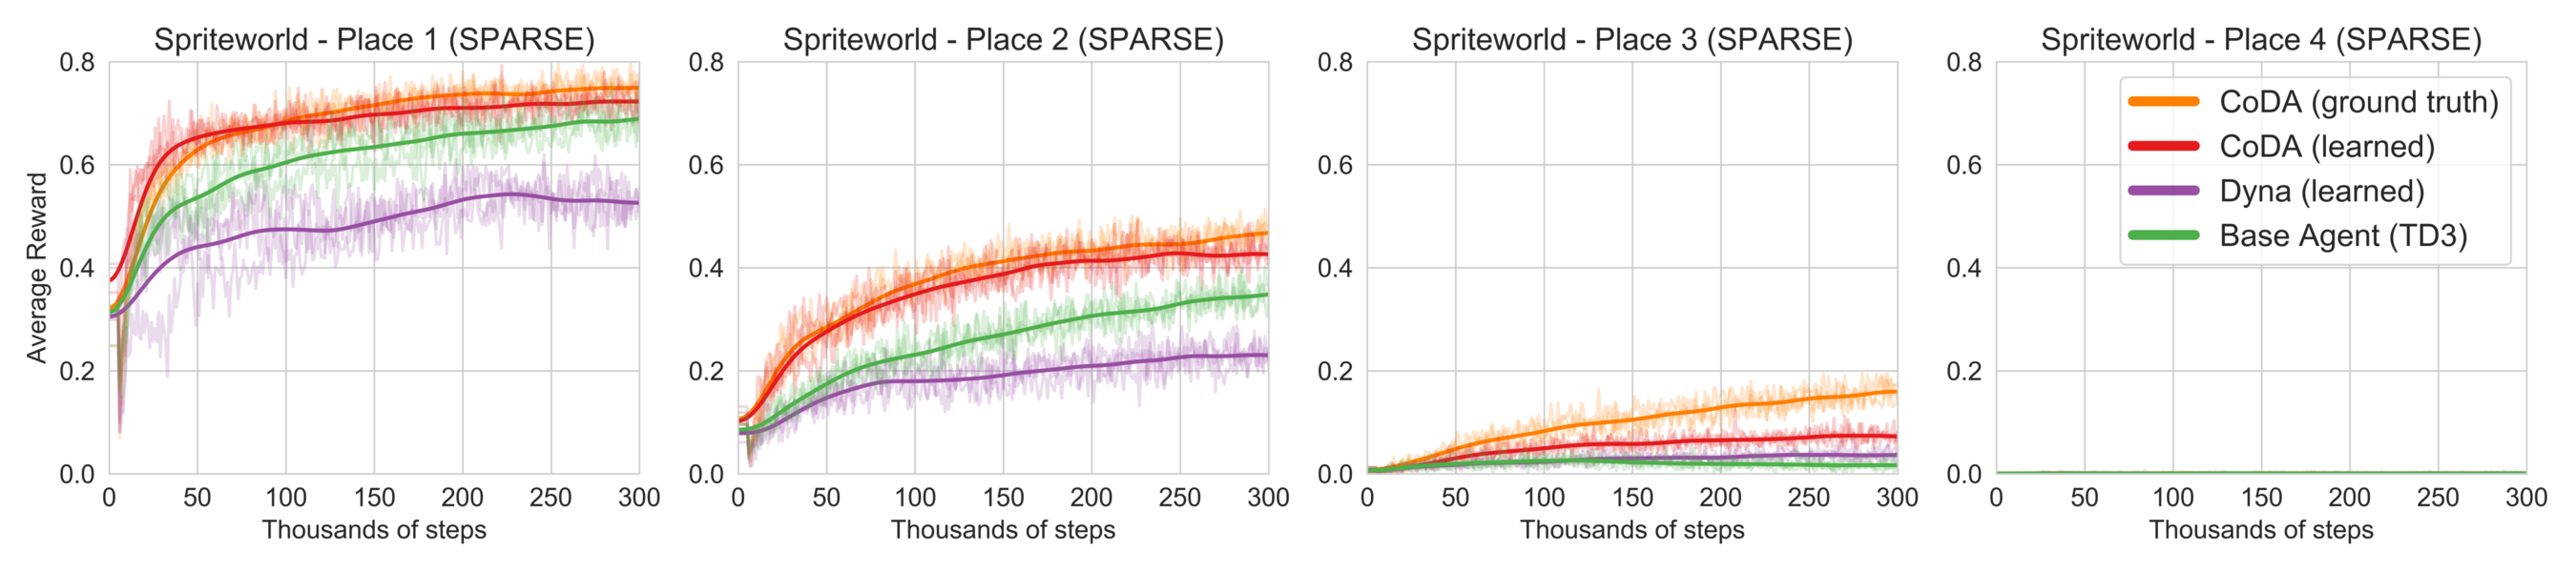
\includegraphics[width=\textwidth]{diagrams/rl_results_plot_sparse.png}
	\caption{\textbf{Average reward on Sparse reward bouncing ball environment.} As in the partial reward case (Figure \ref{fig_rl_results_plot}), we observe that CoDA agents outperform the other agents (except in Place 4, where no agent achieves any reward).}
	\label{fig_rl_results_plot_sparse}
\end{figure}


\paragraph{Results plot} The results plot shows the 3 seeds in reduced opacity together with their smoothed mean.


\subsection{Batch RL}
Here we detail the procedure used in the Batch RL experiments in the \texttt{Pong} environment.

\paragraph{Implementation} This experiment works with a different codebase than the Spriteworld experiment, in order to simplify the use of CoDA in a Batch RL setting. Our experiment first builds the agent's dataset (consisting of real data, dyna data and/or CoDA data), then instantiates a TD3 agent by filling its replay buffer with the dataset. The replay buffer is always expanded to include the entire enlarged dataset (for the 5x CoDA ratio at 250,000 data size this means the buffer has 1.5E6 experiences). The agent is run for 500,000 optimization steps.

\paragraph{Hyperparameters} We used similar hyperparameters to the original TD3 codebase, with the following differences:
\begin{itemize}
\item We use a discount factor of $\gamma = 0.98$ instead of 0.99. 
\item Since Pong is a sparse reward task with $\gamma = 0.98$, we clip critic targets to $(-50, 50)$.
\item We use networks of size $(128, 128)$ instead of $(256, 256)$. 
\item As for our Spriteworld experiment, we use a batch size of $1000$. 
\end{itemize}

\paragraph{Environment} We base our \texttt{Pong} environment on \texttt{RoboSchoolPong-v1} \cite{klimov2017roboschool}. The original environment allowed the ball to teleport back to the center after one of the players scored, offered a small dense reward signal for hitting the ball, and included a stray ``timeout'' feature in the agent's state representation. We fix the environment so that the ball does not teleport, and instead have the episode reset every 150 steps, and also 10 steps after either player scores. The environment is treated as continuous and never returns a done signal that is not also accompanied by a \texttt{TimeLimit.truncated} indicator \cite{brockman2016openai}. We change the reward to be strictly sparse, with reward of $\pm 1$ given when the ball is behind one of the players' paddles. Finally, we drop the stray ``timeout'' feature, so that the state space is 12-dimensional, where each set of 4 dimensions is the x-position, y-position, x-velocity, and y-velocity of the corresponding object (2 paddles and one ball). 

\paragraph{Training the CoDA model}
Without access to a ground truth mask, we needed to train a masking function \ref{sec:inferring_local_factorization} to identify local disentanglement. We also forewent the ground truth reward, instead training our own reward classifier. In each case we used the batch dataset given, and so we trained different models for each random seed. For our masking model, we stacked two single-head transformer blocks (without positional encodings) and used the product of their attention masks as the mask. 
Each block consists of query $Q$, key $K$, and value $V$ networks that each have 3-layers of 256 neurons each, with the attention computed as usual \cite{vaswani2017attention,lee2018set}. 
The transformer is trained to minimize the L2 error of the next state prediction given the current state and action as inputs. 
The input is disentangled, and so has shape \texttt{(batch\_size, num\_components, num\_features)}. In each row (component representation) of each sample, features corresponding to other components are set to zero. 
The transformer is trained for 2000 steps with a batch size of 256, Adam optimizer \cite{kingma2014adam} with learning rate of 3e-4 and weight decay of 1e-5. 
For our reward function we use a fully-connected neural network with 1 hidden layer of 128 units. 
The reward network accepts an $(s, a, s')$ tuple as input (not disentangled) and outputs a softmax over the possible reward values of $[-1, 0, 1]$. 
It is trained for 2000 steps with a batch size of 512, Adam optimizer \cite{kingma2014adam} with learning reate of 1e-3 and weight decay of 1e-4. 
All hyperparameters were rather arbitrary (we used the default setting, or in case it did not work, the first setting that gave reasonable results, as was determined by inspection). 
To ensure that our model and reward functions are trained appropriately (i.e., do not diverge) for each seed, we confirm that the average loss of the CoDA model is below 0.005 at the training and that the average loss of the reward model is below 0.1, which values were found by inspection of a prototype run. These conditions were met by all seeds.

When used to produce masks, we chose a threshold of $\tau = 0.02$ by inspection, which seemed to produce reasonable results. A more principled approach would do cross-validation on the available data, as we did for Spriteworld (Appendix \ref{sec:inferring_local_factorization}). 

\paragraph{Tested configurations}

Table \ref{fig_batch_rl_and_fetch} reports a subset of our tested configurations. We report our results in full below. We considered the following configurations:
\begin{enumerate}
    \item \textbf{Real data only}.
    \item \textbf{CoDA + real data}: after training the CoDA model, we expand the base dataset by either 2, 3, 4 or 6 times.
    \item \textbf{Dyna (using CoDA model)}: after training the CoDA model, we use it as a forward dynamics model instead of for CoDA; we use 1-step rollouts with random actions from random states in the given dataset to expand the dataset by 2x. We also tried with 5-step rollouts, but found that this further hurt performance (not shown).  Note that Dyna results use only 5 seeds.
    \item \textbf{Dyna (using MBPO model)}: as the CoDA model exhibits significant model bias when used as a forward dynamics model, we replicate the state-of-the-art model-based architecture used by MBPO \cite{janner2019trust} and use it as a forward dynamics model for Dyna; we experimented with 1-step and 5-step rollouts with random actions from random states in the given dataset to expand the dataset by 2x. This time we found that the 5-step rollouts do better, which we attribute to the lower model bias together with the ability to create a more diverse dataset (1-step not shown). The MBPO model is described below. We use the same reward model as CoDA to relabel rewards for the MBPO model, which only predicts next state. 
    \item \textbf{MBPO + CoDA}: as MBPO improved performance over the baseline (real data only) at lower dataset sizes, we considered using MBPO together with CoDA. We use the base dataset to train the MBPO, CoDA, and reward models, as described above. We then use the MBPO model to expand the base dataset by 2x, as described above. We then use the CoDA model to expand \textit{the expanded dataset} by 3x the original dataset size. Thus the final dataset is 5x as large as the original dataset (1 real : 1 MBPO : 3 CoDA). 
\end{enumerate}

All configurations alter only the training dataset, and the same agent architecture/hyperparameters (reported above) are used in each case. 

\paragraph{MBPO model}

Since using the CoDA model for Dyna harms rather than helps, we consider using a stronger, state-of-the-art model-based approach. In particular, we adopt the model used by Model-Based Policy Optimization \cite{janner2019trust}. This model consists of a size 7 ensemble of neural networks, each with 4 layers of 200 neurons. We use ReLU activations, Adam optimizer \cite{kingma2014adam} with weight decay of 5e-5, and have each network output a the mean and (log) diagonal covariance of a multi-variate Gaussian. We train the networks with a maximum likelihood loss. To sample from the model, we choose an ensemble member uniformly at random and sample from its output distribution, as in \cite{janner2019trust}. 

\paragraph{Full results}

See Table \ref{table_appendix_batch_rl} for results.

\begin{adjustbox}{center,captionbelow={
Extended Batch RL results. 
Mean success ($\pm$ standard error, estimated using 1000 bootstrap resamples) on \texttt{Pong} environment. All results average over 10 seeds, except Dyna, which uses 5. 
},label=table_appendix_batch_rl,float=table}
\newcommand{\smol}[1]{{\scriptsize\texttt{#1}}}
\centering\small
\begin{tabular}{c@{\hskip 0.2in}ccc@{\hskip 0.16in}|@{\hskip 0.16in}ccccc}
	\toprule
$|\mathcal{D}|$	&Real data& Dyna & MBPO&
\multicolumn{5}{c}{Ratio of Real:CoDA [:MBPO] data (ours)}\\
$(1000s)$ &   1\smol{R}  &   1\smol{R}:1\smol{M} & 1\smol{R}:1\smol{M} &  1\smol{R}:1\smol{C} & 1\smol{R}:2\smol{C}   &  1\smol{R}:3\smol{C}  &  1\smol{R}:5\smol{C} & 1\smol{R}:3\smol{C}:1\smol{M} \\
	\midrule
$\hphantom{0}25$ & $13.2 \pm 0.7$  & $12.2 \pm 1.4$  & $18.5 \pm 1.5$  & $43.8 \pm 2.7$  & $41.6 \pm 3.7$  & $40.9 \pm 2.5$  & $38.4 \pm 4.9$  & $\mybm{46.8} \pm 3.2$  \\
$\hphantom{0}50$ & $22.8 \pm 3.2$  & $17.4 \pm 3.0$  & $36.6 \pm 4.0$  & $66.6 \pm 3.7$  & $58.4 \pm 4.7$  & $64.4 \pm 3.1$  & $62.5 \pm 3.5$  & $\mybm{70.4} \pm 3.7$  \\
$\hphantom{0}75$ & $43.2 \pm 4.7$  & $23.3 \pm 4.7$  & $46.0 \pm 4.5$  & $73.4 \pm 2.8$  & $71.6 \pm 3.8$  & $\mybm{76.7} \pm 2.6$  & $75.0 \pm 3.3$  & $74.6 \pm 3.3$  \\
$100$ & $63.0 \pm 3.0$  & $25.9 \pm 7.4$  & $66.4 \pm 5.2$  & $77.8 \pm 2.0$  & $77.4 \pm 1.8$  & $\mybm{82.7} \pm 1.5$  & $76.6 \pm 3.0$  & $73.7 \pm 2.9$  \\
$150$ & $77.4 \pm 1.3$  & $34.1 \pm 1.5$  & $72.6 \pm 5.6$  & $82.2 \pm 1.7$  & $84.0 \pm 1.2$  & $\mybm{85.8} \pm 1.4$  & $84.2 \pm 1.0$  & $79.7 \pm 3.5$  \\
$250$ & $78.2 \pm 2.7$  & $44.2 \pm 4.0$  & $77.9 \pm 2.3$  & $85.0 \pm 2.8$  & $\mybm{88.1} \pm 1.0$  & $87.8 \pm 1.7$  & $87.0 \pm 1.0$  & $78.3 \pm 5.0$  \\
	\bottomrule\vspace{-0.05in}
\end{tabular}
\end{adjustbox}

\subsection{Goal-conditioned RL}

Here we detail the procedure used in the Goal-conditioned RL experiments on the \texttt{Fetchpush-v1} and \texttt{Slide2} environments.

\paragraph{Implementation} This experiment uses the same codebase as our Batch RL, which provides state-of-the-art baseline HER agents and will be released with the paper.

\paragraph{Hyperparameters}
For \texttt{Fetchpush-v1} we use the default hyperparameters from the codebase, which outperform the original HER agents of \cite{andrychowicz2017hindsight,plappert2018multi} and follow-up works. We do not tune the CoDA agent (but see additional CoDA hyperparameters below). They are as follows:
\begin{itemize}
\item Off-policy algorithm: DDPG \cite{lillicrap2015continuous}
\item Hindsight relabeling strategy:  \texttt{futureactual\_2\_2} \cite{pitisprotoge}, using exclusively \texttt{future} \cite{andrychowicz2017hindsight} relabeling for the first 25,000 steps
\item Optimizer: Adam \cite{kingma2014adam} with default hyperparameters
\item Batch size: 2000
\item Optimization frequency: 1 optimization step every 2 environment steps after the 5000th environment step
\item Target network updates: update every 10 optimization steps with a Polyak averaging coefficient of 0.05
\item Discount factor: 0.98
\item Action l2 regularization: 0.01
\item Networks: 3x512 layer-normalized \cite{ba2016layer} hidden layers with ReLU activations
\item Target clipping: (-50, 0)
\item Action noise: 0.1 Gaussian noise
\item Epsilon exploration \cite{plappert2018multi}: 0.2, with an initial 100\% exploration period of 10,000 steps
\item Observation normalization: yes
\item Buffer size: 1M
\end{itemize}

On \texttt{Slide2} we tried to tune the baseline hyperparameters somewhat, but note that this is a fairly long experiment (10M timesteps) and so only a few settings were tested due to constraints. In particular, we considered the following modifications:
\begin{itemize}
\item Expanding the replay buffer to 2M (effective)
\item Reducing the batch size to 1000 (effective)* (used for results)
\item Using the \texttt{future\_4} strategy (agent fails to learn in 10M steps)
\item Reducing optimization step frequency to 1 step every 4 environment steps (about the same performance)
\end{itemize}

We tried similar adjustments to our CoDA agent, but found the default hyperparameters (used for results) performed well. We found that the CoDA agent outperforms the base HER agent on all tested settings.

For CoDA, we used the following additional  hyperparameters:
\begin{itemize}
\item CoDA buffer size: 3M
\item Make CoDA data every: 250 environment steps
\item Number of source pairs from replay buffer used to make CoDA data: 2000
\item Number of CoDA samples per source pair: 2
\item Maximum ratio of CoDA:Real data to train on: 3:1
\end{itemize}
\paragraph{Environment} 

\begin{wrapfigure}{r}{0.23\textwidth}
    \vspace{-\baselineskip}
	\centering
    \captionsetup{width=0.22\textwidth}
	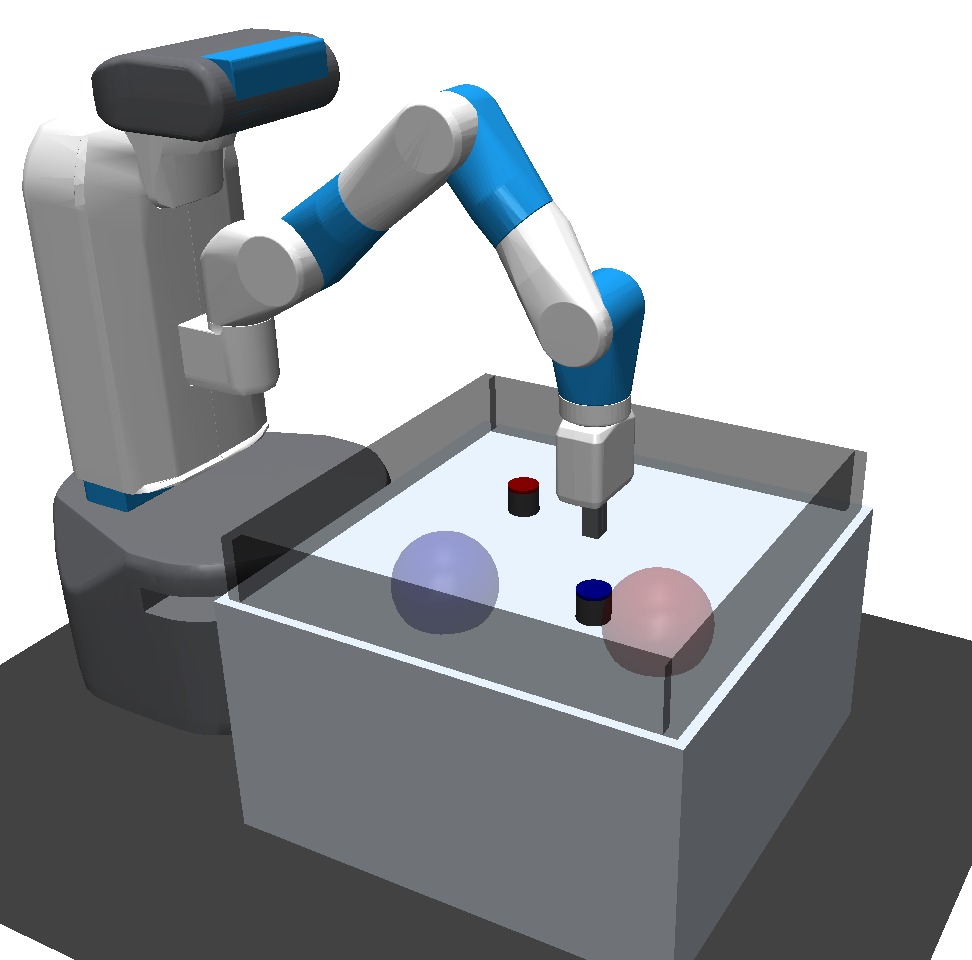
\includegraphics[width=0.22\textwidth,height=0.2\textwidth]{diagrams/env_fetch.png}
	\caption{The \texttt{Slide2} environment.}
	\label{fig_env_fetch_appendix}
    \vspace{-\baselineskip}
\end{wrapfigure}

On \texttt{FetchPush-v1} the standard state features include the relative position of the object and gripper, which entangles the two. While this could be dealt with by dynamic relabeling (as used for HER's reward), we simply drop the corresponding features from the state. 

\texttt{Slide2} has two pucks that slide on a table and bounce off of a solid railing. Observations are 40-dimensional (including the 6-dimensional goal), and actions are 4-dimensional. Initial positions and goal positions are sampled randomly on the table. During training, the agent gets a sparse reward of 0 (otherwise -1) if \textit{both} pucks are within 5cm of their ordered target. At test time we count success as having both picks within 7.5cm of the target on the last step of the episode. Episodes last 75 steps and there is no done signal (this is intended as a continuous task).

\paragraph{CoDA Heuristic} For these experiments we use a hand-coded heuristic designed with domain knowledge. In particular, we assert that the action is always entangled with the gripper, and that gripper/action and objects (pucks or blocks) are disentangled whenever they are more than 10cm apart. This encodes independence due to physical separation, which we hypothesize is a very generally heuristic that humans implicitly rely on all the time.  The pucks have a radius of 2.5cm and height of 4cm, and the blocks are 5cm x 5cm x 5cm, so this heuristic is quite generous / suboptimal. Despite being suboptimal, it demonstrates the ease with which domain knowledge can be injected via the CoDA mask: we need only a high precision (low false positive rate) heuristic---the recall is not as important. It is likely that an agent could learn a better mask that also takes into account velocity.

\paragraph{Results plot} The plot shows mean $\pm 1$ standard deviation of the smoothed data over 5 seeds.

\end{document}